\par{Listing \ref{more_work_kernel} its our attempt to give every \emph{work item} more computational load, that way decreasing the
    effects of scheduling and spawning overhead of \emph{work items} and \emph{work groups}. This way the behaviour when cycles 
    per \emph{work item} are increased can be studied. This was achieved changing the dimension of the \emph{NDRange} from 2 to 1
    and making that every instance of a \emph{kernel} calculate the results of several of the elements of the resulting matrix,
    as it can be seen in line \emph{10} of listing 4.}

\par{Figure \ref{MoreWork} shows that in the case of the Xeon Phi co-processor and the Xeon CPU, the effect of vectorization
    is the same that in the previous kernel(16 for the Xeon Phi and 4 for the Xeon CPU), the other interesting effect in this
    case is the performance degradation after \emph{work group} dimension 64x64 on the Xeon Phi and after 128x128 on the Xeon
    CPU, clearly the Xeon Phi is more sensible to the decreasing number of \emph{work groups} than the Xeon CPU, one of the 
    reasons for this is the number of \emph{computation units} available in these 2 architectures, on the Xeon Phi is 236 and
    on the Xeon CPU is 40, as the number of \emph{work groups} decreased, as it is shown on table \ref{tab:work_groups}, the amount
    of available parallelism that take advantage of the \emph{comput units} available in these 2 architectures decreases as well.}


\par{{\color{red}EVERY WORK ITEM IT IS IN CHARGE OF ONE ROW!!!!!!!!!!!!!!!!!!!!!!!!!!}}

\begin{figure}[!h]
    \centering
    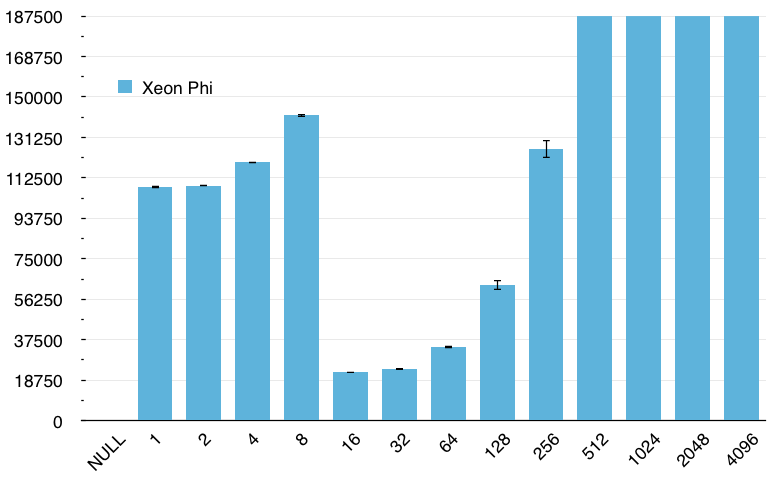
\includegraphics[width=0.49\textwidth]{figures/opt1_phi.png}
    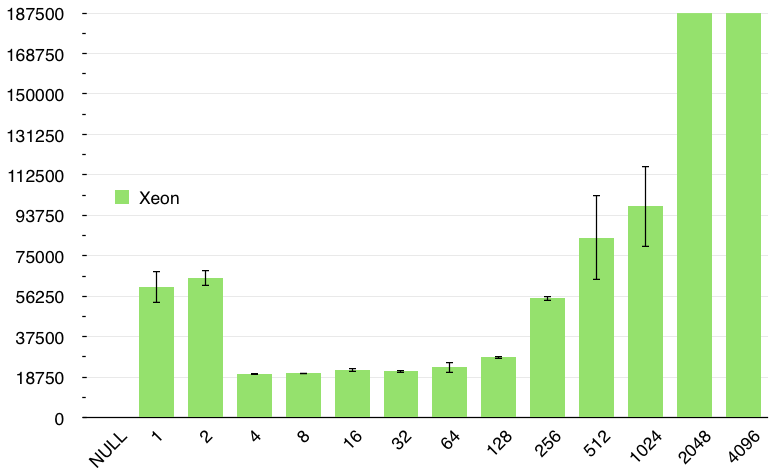
\includegraphics[width=0.49\textwidth]{figures/opt1_cpu.png}
    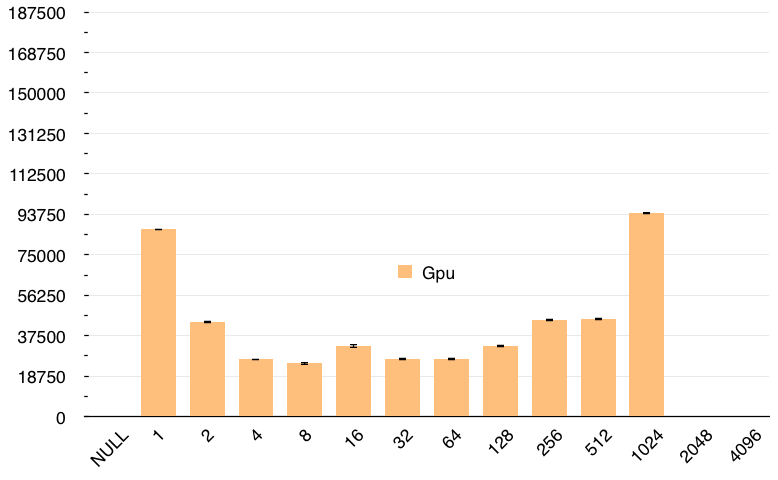
\includegraphics[width=0.49\textwidth]{figures/opt1_gpu.png}
    \caption{Matrix multiplication with more work in different architectures.}
    \label{MoreWork}
\end{figure}

\begin{table}[!h]
    \centering
    \begin{tabular}{| l | l | l | l |}
    \hline
    \emph{Work Group} Dimension & \#\emph{Work Groups} \\ \hline
    16 & 256 \\ \hline
    32 & 128 \\ \hline
    64 & 64 \\ \hline
    128 & 32 \\ \hline
    256 & 16 \\ \hline
    512 & 8 \\ \hline
    1024 & 4 \\ \hline
    2048 & 2 \\ \hline
    4096 & 1 \\ 
    \hline
    \end{tabular}
    \caption{\emph{Work group} dimension versus numbers of \emph{work groups}.}
    \label{tab:work_groups}
\end{table}

\par{In this case the most performant of the 3 architectures analized is the Xeon as its shown on figure\ref{MoreWorkRes} and 
    we cannot see any advantage in comparison with the naive \emph{kernel} using more load per \emph{work item}.}

\begin{figure}[!h]
    \centering
    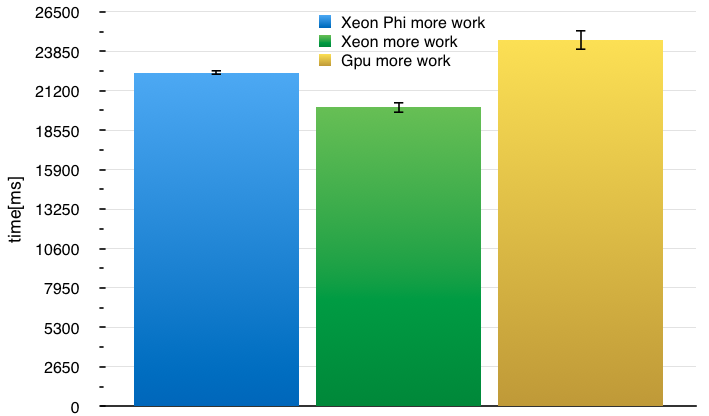
\includegraphics[width=0.49\textwidth]{figures/moreWorkRes.png}
    \caption{Comparison between the best cases of the more work \emph{kernel} in different devices.}
    \label{MoreWorkRes}
\end{figure}

\par{Figures \ref{gpu}\ref{phi}\ref{xeon} is possible to see that the only device that got some performance improvements from this \emph{kernel}
    change was the Xeon.(\emph{explain why})}





